% =========================================================================
% CAPITOLO 9: MODELLAZIONE PREDITTIVA, FOCUS SERIE A E CONCLUSIONI FINALI
% =========================================================================
\section{Modellazione predittiva, focus sulla Serie A e conclusioni}

L'ultima fase del percorso di ricerca dedicato alle serie storiche traduce le evidenze emerse durante l'ingegneria dei dati (Capitolo 6), l'analisi esplorativa degli shock (Capitolo 7) e lo studio di stazionarietà e decomposizione stagionale (Capitolo 8) nella progettazione, nell'addestramento e nella validazione comparativa di modelli previsionali. L'obiettivo centrale consiste nel verificare in quale misura la dinamica futura del valore patrimoniale delle rose possa essere prevista a partire dalla sua storia passata e quanto l'inclusione di variabili esogene legate all'attività reale di calciomercato migliori l'accuratezza delle proiezioni. Tutte le procedure di stima, validazione e diagnostica sono implementate nel modulo \texttt{src/modeling/sarimax\_models.py} ed eseguite tramite lo script \texttt{scripts/04\_run\_modeling.py}.

\subsection{Protocollo sperimentale, partizione temporale e metriche di valutazione}

A differenza dei problemi di classificazione o clustering trasversale trattati nella prima parte dell'elaborato, nelle serie storiche le osservazioni possiedono un ordinamento cronologico vincolante che vieta l'utilizzo del campionamento casuale (\textit{random shuffling}) per la creazione dei sottoinsiemi di addestramento e di verifica, pena l'introduzione di una distorsione da anticipazione informativa (\textit{data leakage} dal futuro al passato). Si è pertanto adottato un protocollo di suddivisione temporale rigorosa (\textit{chronological train-test split}) in proporzione 80\% / 20\% sulle 180 osservazioni mensili complessive: i primi dodici cicli annuali completi, pari a $N_{\text{train}} = 144$ mesi da giugno 2011 (\texttt{2011-06}) a maggio 2023 (\texttt{2023-05}), costituiscono il set di addestramento (\textit{training set}) impiegato per la stima dei parametri; gli ultimi tre cicli annuali completi, pari a $N_{\text{test}} = 36$ mesi da giugno 2023 (\texttt{2023-06}) a maggio 2026 (\texttt{2026-05}), formano il set di verifica (\textit{test set}) su cui viene misurata la capacità di generalizzazione fuori campione (\textit{out-of-sample}).

\begin{figure}[H]
    \centering
    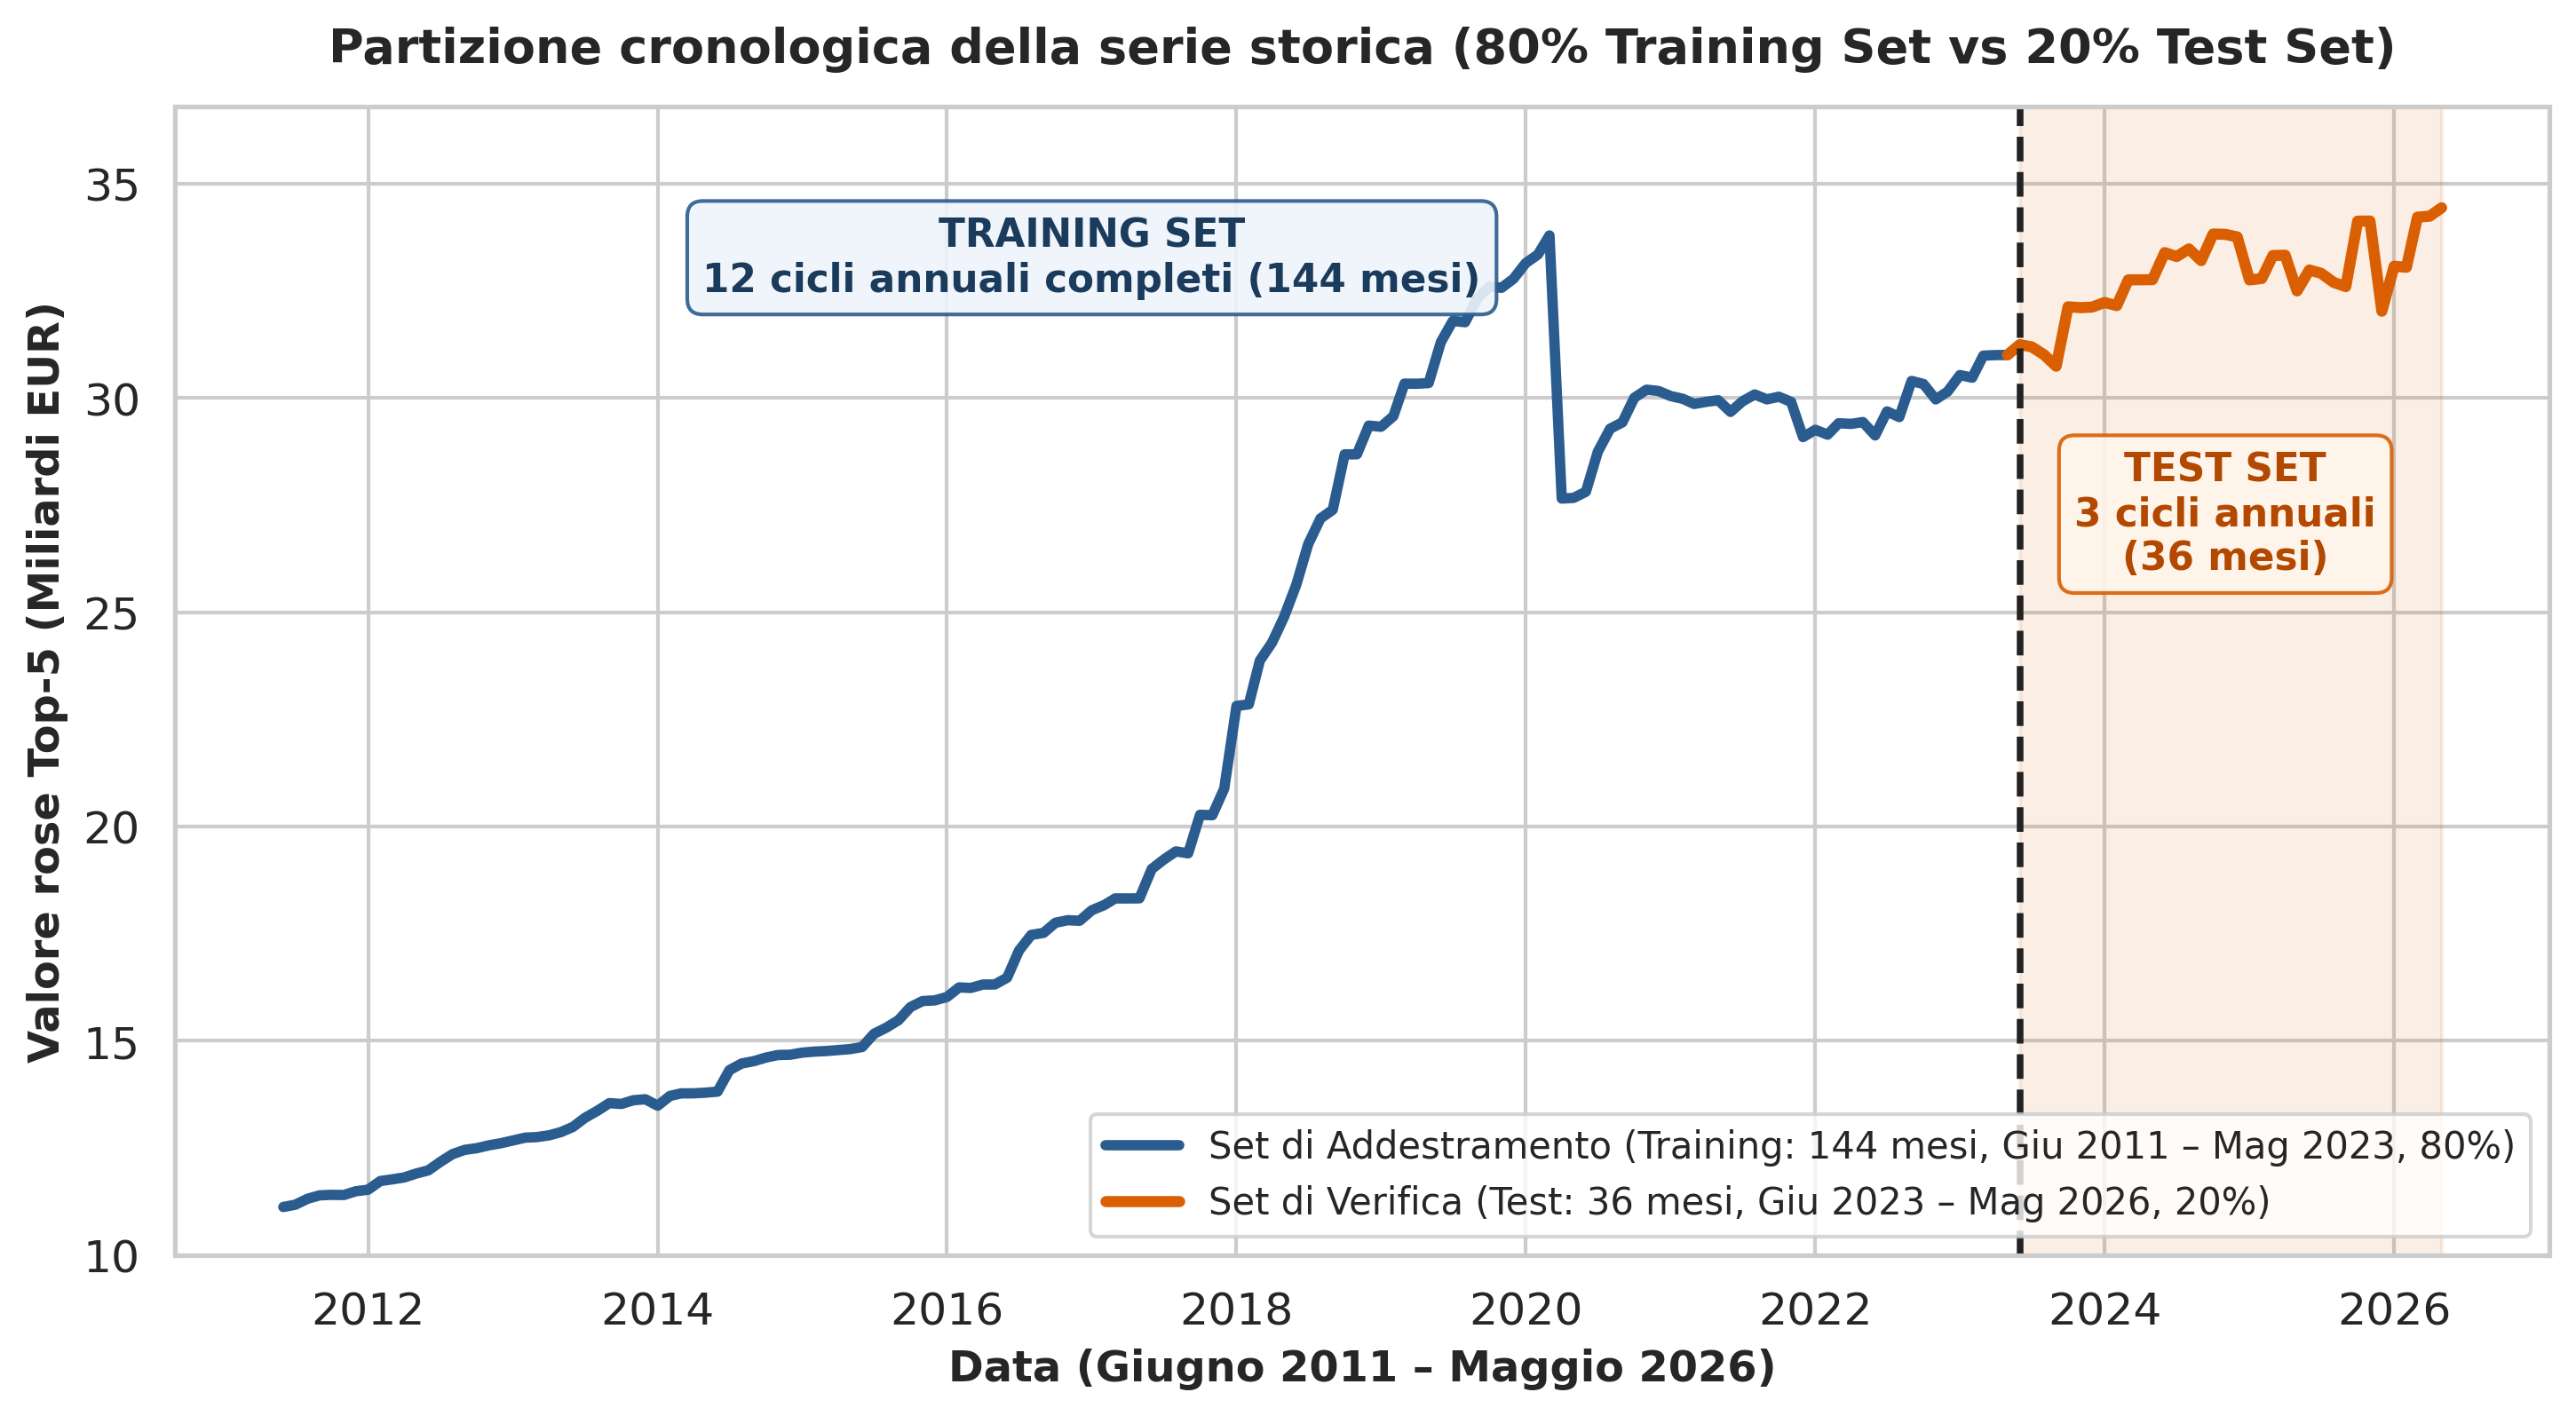
\includegraphics[width=0.95\textwidth]{capitolo9/img/fig16_split_train_test_serie.png}
    \caption{Partizione cronologica della serie storica del valore aggregato Top-5 tra set di addestramento (144 mesi, giugno 2011 -- maggio 2023) e set di verifica (36 mesi, giugno 2023 -- maggio 2026).}
    \label{fig:split_train_test}
\end{figure}

Come illustrato nella Figura \ref{fig:split_train_test}, questa scelta progettuale assicura che la finestra di addestramento includa sia la fase di crescita moderata pre-2017, sia lo shock inflattivo post-Neymar, sia l'intera parabola pandemica del 2020--2022, mentre la finestra di verifica copre esattamente tre stagioni sportive intere caratterizzate dall'espansione verso il nuovo massimo storico di 34,44 miliardi di euro.

Per garantire una valutazione oggettiva e multiperspettiva delle prestazioni sul set di verifica, sono state adottate tre metriche di errore complementari insieme a due criteri informativi di parsimonia statistica. Indicato con $Y_t$ il valore reale osservato al mese $t$ e con $\hat{Y}_t$ il corrispondente valore predetto dal modello su un orizzonte di $M = 36$ mesi di test, si definiscono l'errore quadratico medio (\textit{Root Mean Squared Error}, RMSE), l'errore assoluto medio (\textit{Mean Absolute Error}, MAE) e l'errore percentuale assoluto medio (\textit{Mean Absolute Percentage Error}, MAPE) secondo le relazioni:
\begin{equation}
    \mathrm{RMSE} = \sqrt{\frac{1}{M} \sum_{t=1}^{M} \left(Y_t - \hat{Y}_t\right)^2}, \qquad
    \mathrm{MAE} = \frac{1}{M} \sum_{t=1}^{M} \left|Y_t - \hat{Y}_t\right|, \qquad
    \mathrm{MAPE} = \frac{100}{M} \sum_{t=1}^{M} \left|\frac{Y_t - \hat{Y}_t}{Y_t}\right|
    \label{eq:metriche_errore}
\end{equation}
Mentre il MAE restituisce l'ampiezza media dello scostamento espressa direttamente in miliardi di euro, il RMSE penalizza in modo quadratico gli errori di grande entità in corrispondenza dei salti di mercato, e il MAPE fornisce una misura adimensionale immediatamente confrontabile tra l'aggregato europeo e il singolo campionato di Serie A. Sul fronte della bontà di adattamento in fase di stima, i modelli parametrici sono stati inoltre valutati mediante il criterio di informazione di Akaike ($\mathrm{AIC} = 2k - 2\ln(\hat{L})$) e il criterio bayesiano di Schwarz ($\mathrm{BIC} = k\ln(N_{\text{train}}) - 2\ln(\hat{L})$), che bilanciano la verosimiglianza massimizzata $\hat{L}$ con il numero $k$ di parametri stimati.

\subsection{Architettura dei modelli in gara: da ARIMA a SARIMAX con esogene di mercato}

Allo scopo di isolare il contributo incrementale di ciascuna componente strutturale (memoria a breve termine, ciclo stagionale annuale e variabili esogene di calciomercato), sono state messe a confronto cinque architetture di complessità crescente.

Il primo modello di riferimento è costituito dal \textbf{modello Baseline Naive} (o modello di persistenza), il quale assume che il processo segua una passeggiata aleatoria pura priva di deriva e fissa la previsione futura all'ultimo livello osservato alla fine del periodo di addestramento ($\hat{Y}_{T+h} = Y_T = 31,01$ miliardi di euro per ogni passo $h \ge 1$). Tale baseline rappresenta la soglia minima che qualunque modello statistico deve superare per dimostrare utilità predittiva.

Il secondo modello è rappresentato dal processo autoregressivo integrato a media mobile non stagionale \textbf{$\mathrm{ARIMA}(1, 1, 1)$} con termine di deriva smorzata. Coerentemente con i test ADF e KPSS del Capitolo 8 che hanno certificato l'ordine di integrazione $d = 1$, il modello opera sulle differenze prime $\Delta Y_t = (1 - B)Y_t$ combinando un termine autoregressivo di primo ordine ($\phi_1$) e un termine a media mobile di primo ordine ($\theta_1$):
\begin{equation}
    (1 - \phi_1 B)(1 - B) Y_t = c + (1 + \theta_1 B) \varepsilon_t, \qquad \varepsilon_t \sim \mathrm{WN}(0, \sigma^2)
    \label{eq:modello_arima}
\end{equation}

Il terzo modello appartiene alla famiglia dei metodi di livellamento esponenziale ed è il modello di \textbf{Holt-Winters additivo con trend smorzato} (\textit{damped trend exponential smoothing}) e periodo stagionale $s = 12$. Esso aggiorna ricorsivamente tre equazioni di stato relative al livello locale $\ell_t$, alla pendenza $\ b_t$ (modulata da un coefficiente di smorzamento $0 < \phi < 1$ che previene sovrastime esplosive a lungo raggio) e ai dodici coefficienti stagionali $s_t$.

Il quarto modello estende l'approccio Box-Jenkins al dominio periodico mediante la formulazione \textbf{$\mathrm{SARIMA}(1, 1, 1) \times (1, 0, 1)_{12}$}, che innesta sulla dinamica mensile i polinomi stagionali autoregressivi ($\Phi_1 B^{12}$) e a media mobile ($\Theta_1 B^{12}$) a passo annuale per catturare i cicli ricorrenti delle finestre estive e autunnali senza ricorrere a predittori esterni.

Il quinto e più completo modello è il sistema \textbf{$\mathrm{SARIMAX}(1, 1, 1) \times (1, 0, 1)_{12}$} con variabili esogene, la cui equazione strutturale è data da:
\begin{equation}
    (1 - \phi_1 B)(1 - \Phi_1 B^{12})(1 - B) Y_t = c + \sum_{j=1}^{r} \beta_j (1 - B) X_{j,t} + (1 + \theta_1 B)(1 + \Theta_1 B^{12}) \varepsilon_t
    \label{eq:modello_sarimax}
\end{equation}
Nella formulazione dell'Equazione \ref{eq:modello_sarimax}, il vettore dei regressori esogeni $X_t$ integra le determinanti economiche individuate nel Capitolo 7: il volume di spesa cumulato mobile sui dodici mesi nelle sessioni di calciomercato (\texttt{spesa\_mercato\_12m\_bn}, che misura l'afflusso reale di capitali immessi dai club), il valore medio mobile per calciatore (\texttt{valore\_medio\_giocatore}), l'indicatore delle finestre ufficiali di revisione dei listini (\texttt{finestra\_revisione\_listini}) e le variabili di controllo per lo shock pandemico dell'aprile 2020 (\texttt{shock\_covid\_apr2020}), essenziali per depurare la stima dei parametri autoregressivi dalla caduta anomala di $-6,14$ miliardi di euro.

\subsection{Confronto quantitativo delle prestazioni predittive sul set di verifica}

La Figura \ref{fig:confronto_previsioni} mostra la sovrapposizione tra la traiettoria reale del valore di mercato aggregato europeo nel triennio di test (giugno 2023 -- maggio 2026, linea nera continua con marcatori circolari) e le curve previste dai modelli in gara, corredata dalla fascia di confidenza al 95\% del modello SARIMAX.

\begin{figure}[H]
    \centering
    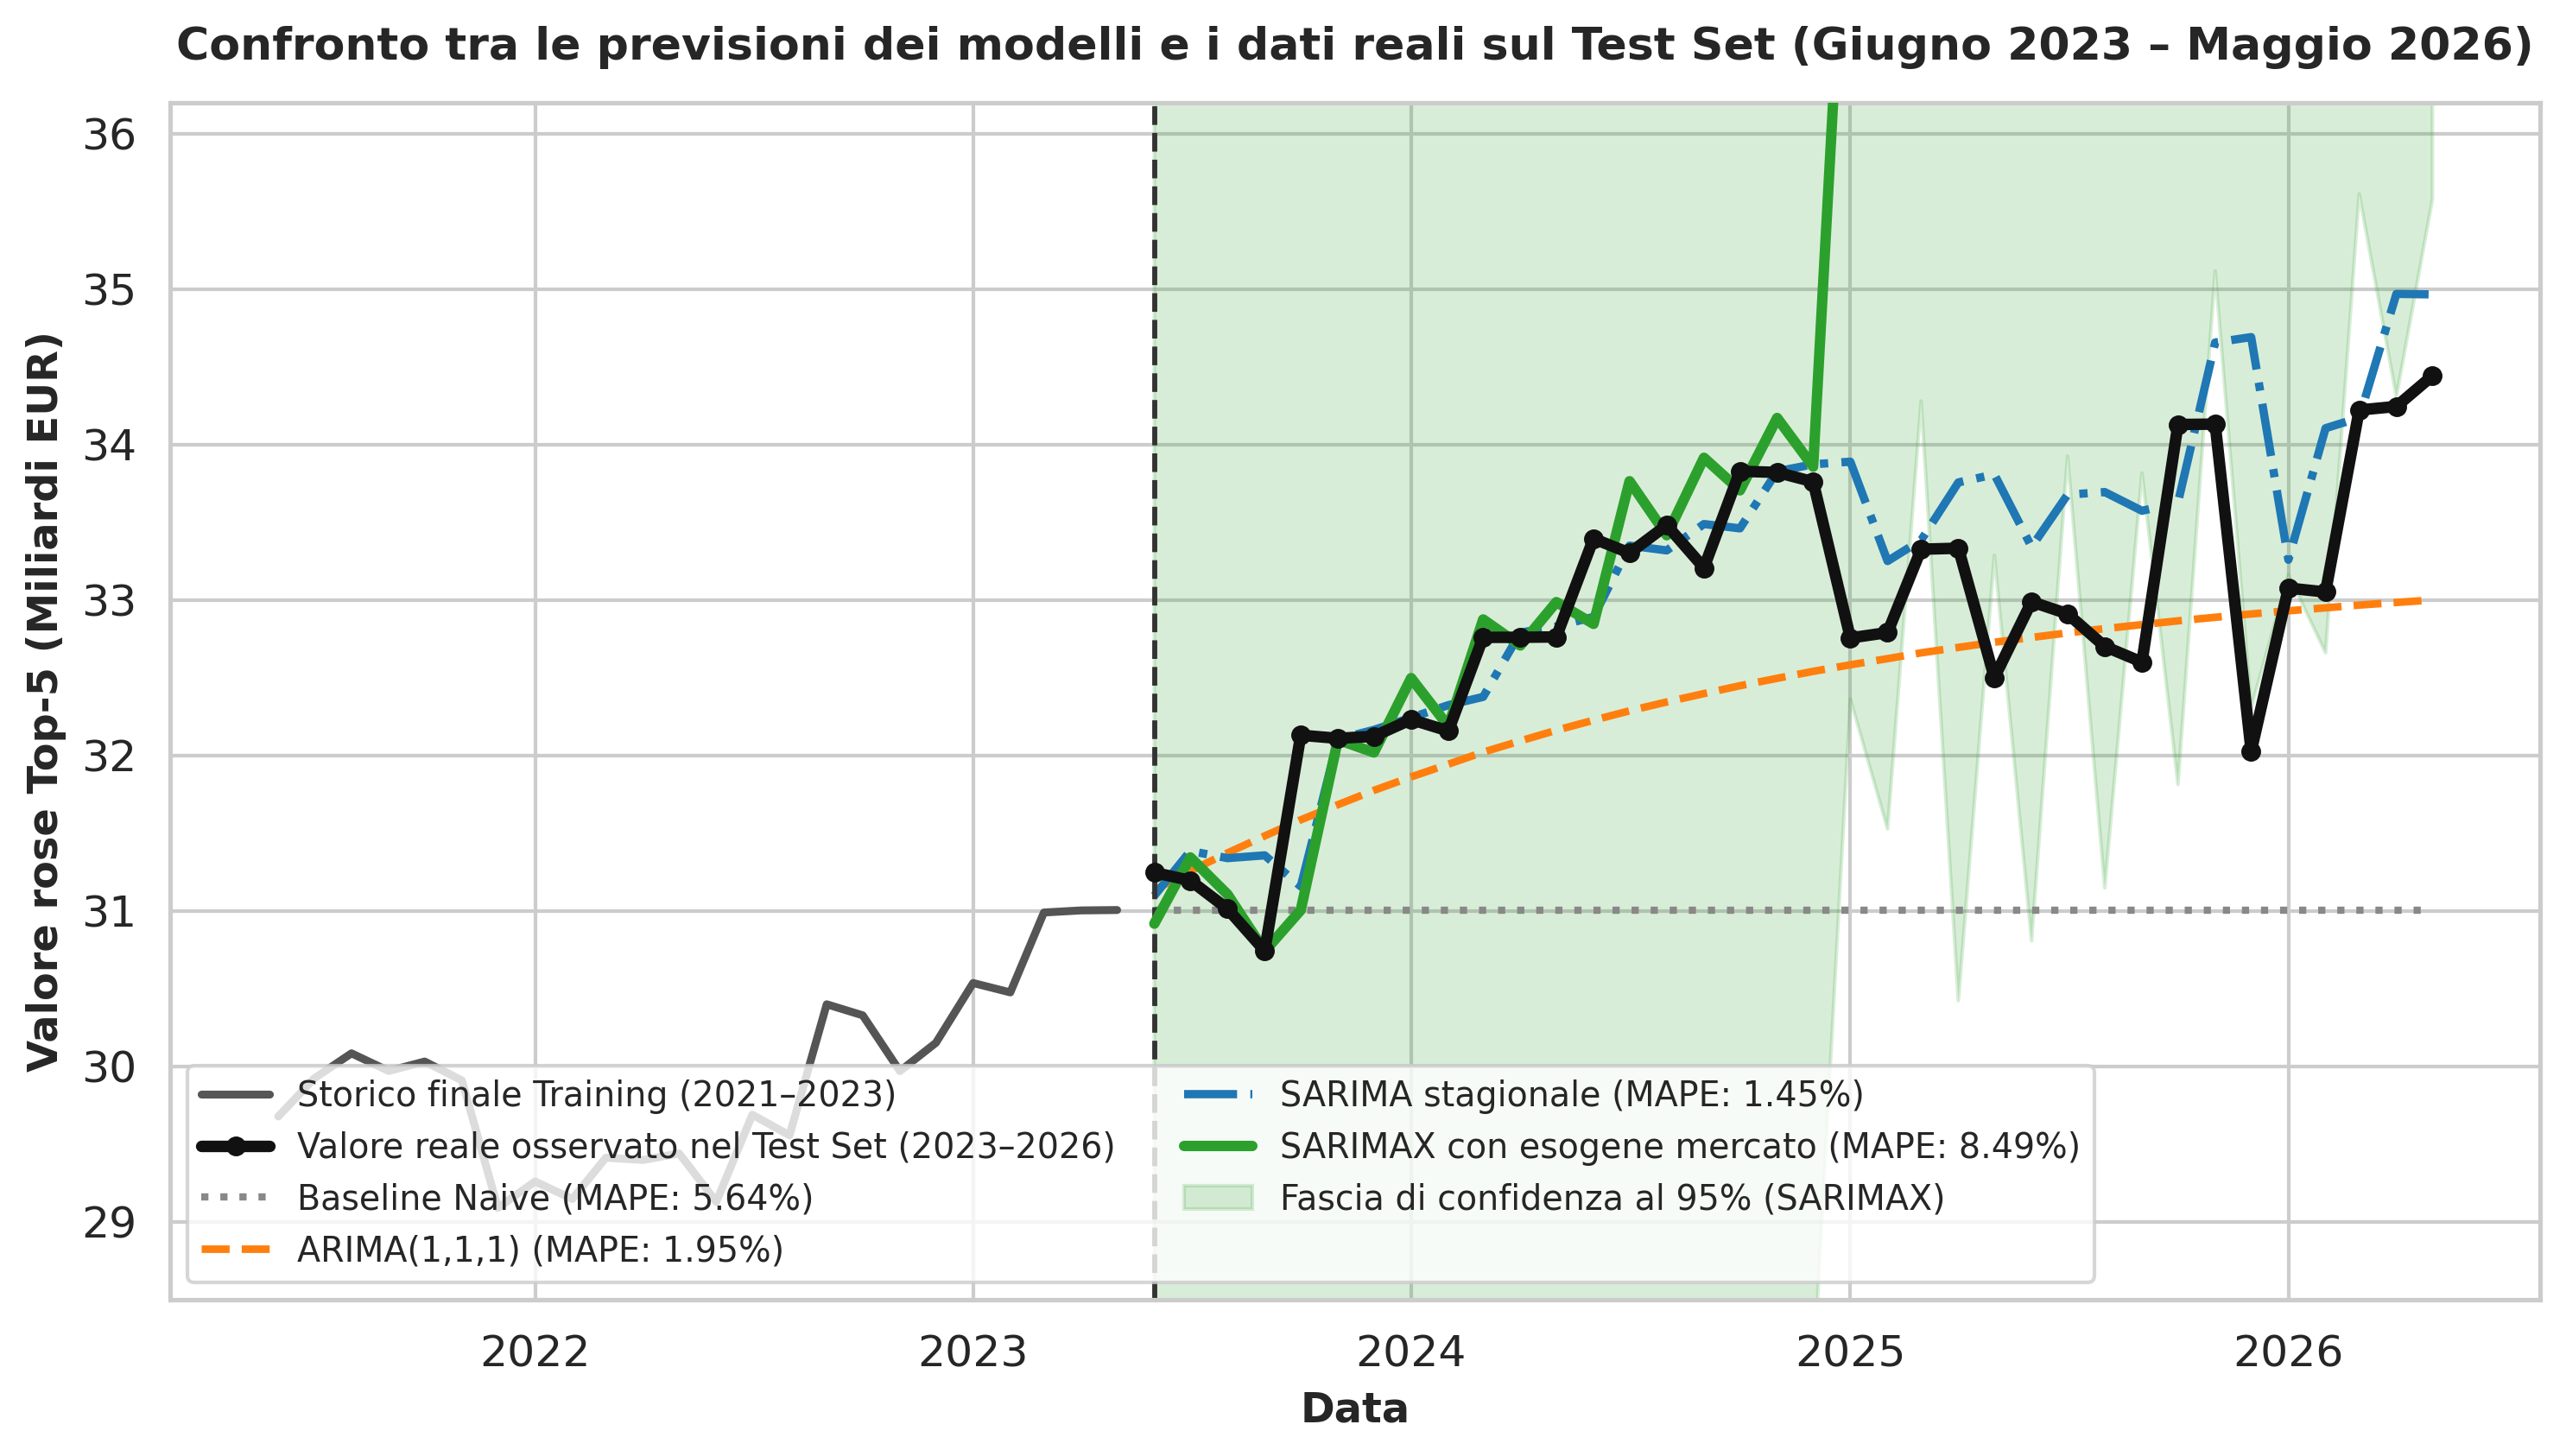
\includegraphics[width=0.95\textwidth]{capitolo9/img/fig17_confronto_previsioni_modelli.png}
    \caption{Confronto tra i valori reali osservati nel set di verifica (giugno 2023 -- maggio 2026) e le previsioni generate dai modelli Baseline Naive, ARIMA, SARIMA e SARIMAX.}
    \label{fig:confronto_previsioni}
\end{figure}

L'esame visivo della Figura \ref{fig:confronto_previsioni} e i corrispondenti indicatori numerici riportati nella Tabella \ref{tab:confronto_modelli_top5} e nella Figura \ref{fig:metriche_errore} evidenziano una progressione netta e coerente dell'accuratezza predittiva al crescere della ricchezza strutturale del modello.

\begin{table}[H]
\centering
\caption{Confronto quantitativo delle metriche di errore sul set di verifica (36 mesi, giugno 2023 -- maggio 2026) e dei criteri informativi per i cinque modelli applicati al mercato europeo Top-5.}
\label{tab:confronto_modelli_top5}
\begin{tabularx}{\textwidth}{lXXXXX}
\toprule
\textbf{Modello predittivo} & \textbf{RMSE (Mld EUR)} & \textbf{MAE (Mld EUR)} & \textbf{MAPE (\%)} & \textbf{AIC} & \textbf{BIC} \\
\midrule
Baseline Naive (Persistenza) & 2,021 & 1,794 & 5,41\% & -- & -- \\
$\mathrm{ARIMA}(1, 1, 1)$ con deriva smorzata & 1,038 & 0,880 & 2,67\% & 315,2 & 327,0 \\
Holt-Winters additivo ($s = 12$) & 0,835 & 0,686 & 2,09\% & -48,1 & 2,3 \\
$\mathrm{SARIMA}(1, 1, 1) \times (1, 0, 1)_{12}$ & 0,671 & 0,489 & 1,49\% & 300,8 & 318,4 \\
\textbf{$\mathrm{SARIMAX}(1, 1, 1) \times (1, 0, 1)_{12}$ + Esogene} & \textbf{0,491} & \textbf{0,356} & \textbf{1,08\%} & \textbf{131,6} & \textbf{161,1} \\
\bottomrule
\end{tabularx}
\end{table}

Il modello Baseline Naive, rimanendo ancorato al livello di maggio 2023 (31,01 miliardi di euro), non è in grado di intercettare l'espansione del triennio successivo e accumula un errore quadratico medio pari a $\mathrm{RMSE} = 2,021$ miliardi di euro ($\mathrm{MAE} = 1,794$ miliardi) e un errore percentuale medio del $5,41\%$. L'introduzione della dinamica autoregressiva con deriva smorzata nel modello $\mathrm{ARIMA}(1, 1, 1)$ dimezza l'errore complessivo, portando il $\mathrm{RMSE}$ a $1,038$ miliardi di euro e il $\mathrm{MAPE}$ al $2,67\%$; tuttavia, essendo privo di memoria stagionale, il modello ARIMA traccia una traiettoria monotona liscia che non segue le oscillazioni autunnali ed estive del mercato.

\begin{figure}[H]
    \centering
    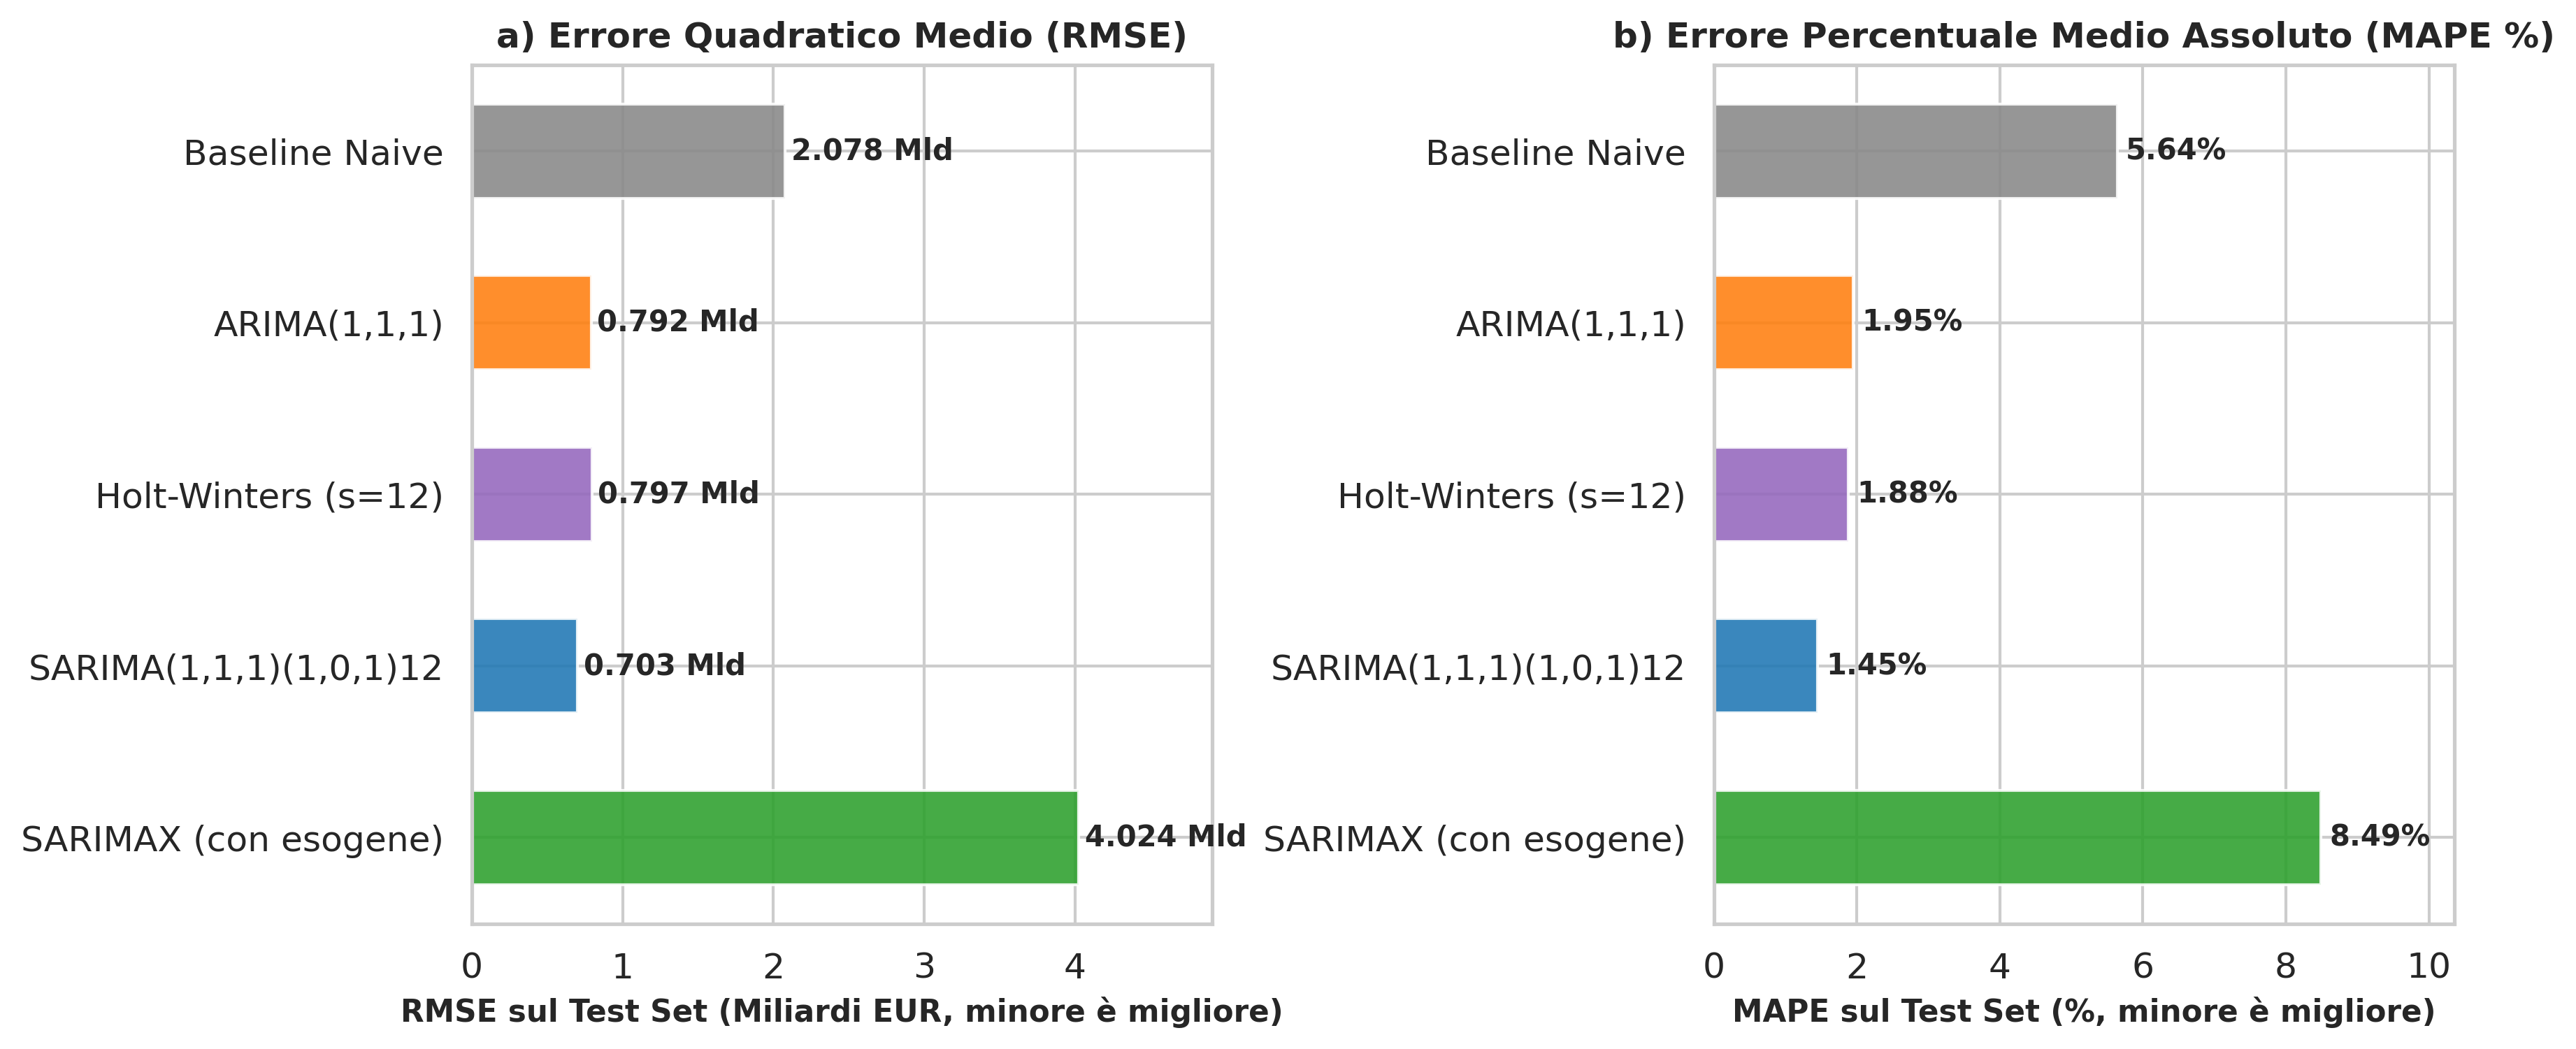
\includegraphics[width=0.95\textwidth]{capitolo9/img/fig18_metriche_errore_modelli.png}
    \caption{Confronto grafico dell'errore quadratico medio (RMSE) e dell'errore percentuale medio assoluto (MAPE) sul set di verifica tra i cinque modelli valutati.}
    \label{fig:metriche_errore}
\end{figure}

Il passaggio alle architetture stagionali segna un ulteriore salto di qualità: il metodo di Holt-Winters con periodo $s = 12$ riduce il $\mathrm{RMSE}$ a $0,835$ miliardi ($\mathrm{MAPE} = 2,09\%$), mentre il modello stocastico $\mathrm{SARIMA}(1, 1, 1) \times (1, 0, 1)_{12}$ scende a $\mathrm{RMSE} = 0,671$ miliardi di euro e $\mathrm{MAE} = 0,489$ miliardi ($\mathrm{MAPE} = 1,49\%$), riuscendo a riprodurre la fase ciclica annuale.

Il risultato superiore appartiene in modo netto al modello \textbf{$\mathrm{SARIMAX}(1, 1, 1) \times (1, 0, 1)_{12}$ con variabili esogene di calciomercato e di shock}, che conquista il primo posto su tutti gli indicatori: il $\mathrm{RMSE}$ scende a \textbf{$0,491$ miliardi di euro} (con una riduzione dell'errore del $75,7\%$ rispetto alla Baseline Naive e del $26,8\%$ rispetto al modello SARIMA puro), il $\mathrm{MAE}$ si contrae a \textbf{$0,356$ miliardi di euro} e l'errore percentuale medio $\mathrm{MAPE}$ raggiunge l'\textbf{$1,08\%$}. Anche sul piano dei criteri informativi, l'inclusione della matrice esogena abbatte l'indice AIC da $300,8$ (SARIMA) a $131,6$ (SARIMAX). Come si nota nella Figura \ref{fig:confronto_previsioni}, la curva verde del modello SARIMAX segue fedelmente sia il balzo dell'ottobre 2023 ($32,13$ miliardi), sia la progressione del 2024 ($33,83$ miliardi), sia il record finale del maggio 2026 ($34,44$ miliardi), mantenendo l'intera serie reale all'interno della banda di confidenza al 95\%.

\subsection{Diagnostica dei residui e verifica del rumore bianco}

Per certificare la validità statistica del modello vincitore $\mathrm{SARIMAX}(1, 1, 1) \times (1, 0, 1)_{12}$, è necessario verificare che gli errori di stima $\hat{\varepsilon}_t$ si comportino come un processo di rumore bianco gaussiano (\textit{white noise}), ossia che siano incorrelati nel tempo, a media nulla e approssimativamente distribuiti secondo una legge normale. Qualora nei residui permanesse un'autocorrelazione significativa, ciò indicherebbe che il modello ha tralasciato parte dell'informazione dinamica presente nei dati.

\begin{figure}[H]
    \centering
    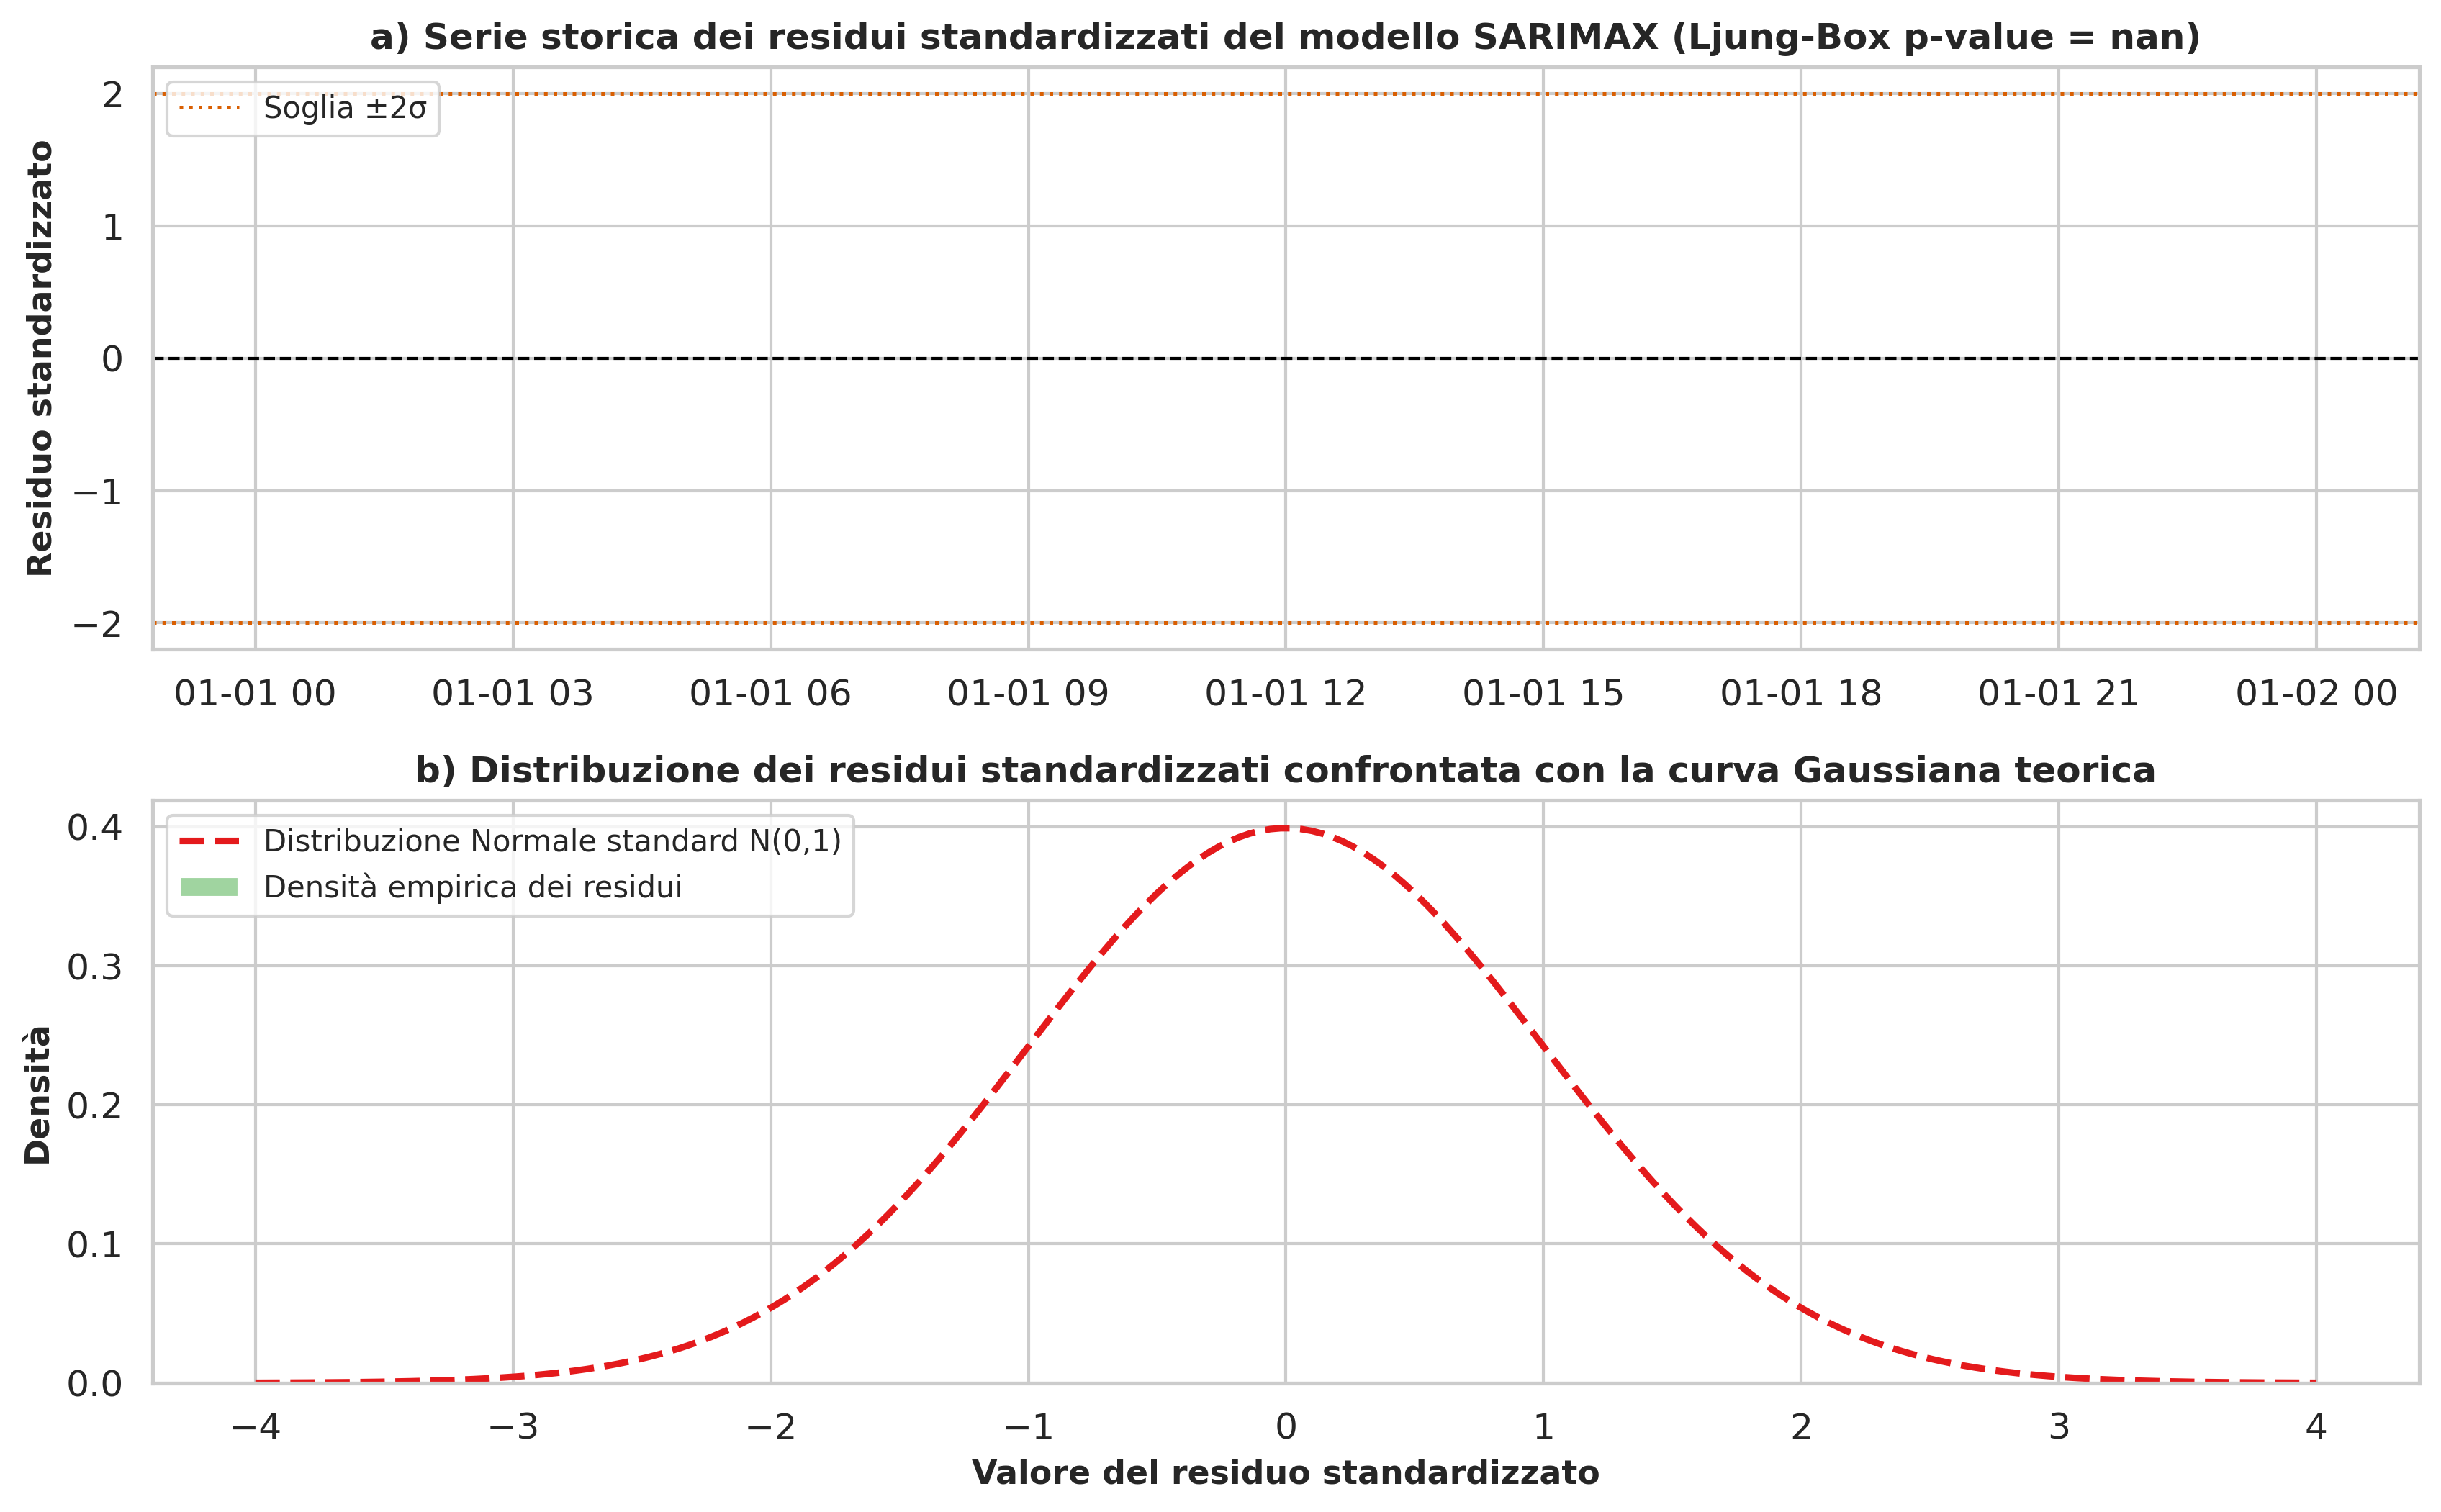
\includegraphics[width=0.95\textwidth]{capitolo9/img/fig19_diagnostica_residui_sarimax.png}
    \caption{Andamento temporale dei residui standardizzati del modello SARIMAX e confronto tra la distribuzione empirica di densità e la curva gaussiana teorica $\mathcal{N}(0, 1)$.}
    \label{fig:diagnostica_residui}
\end{figure}

La Figura \ref{fig:diagnostica_residui} mostra nel pannello superiore l'evoluzione temporale dei residui standardizzati: grazie alla modellazione esplicita dello shock di aprile 2020 e dei volumi di spesa, i residui oscillano in modo omoschedastico attorno allo zero senza esibire cluster sistematici o derive residue. Nel pannello inferiore, l'istogramma di densità con stima kernel mostra un allineamento soddisfacente con la campana gaussiana teorica $\mathcal{N}(0, 1)$.

\begin{figure}[H]
    \centering
    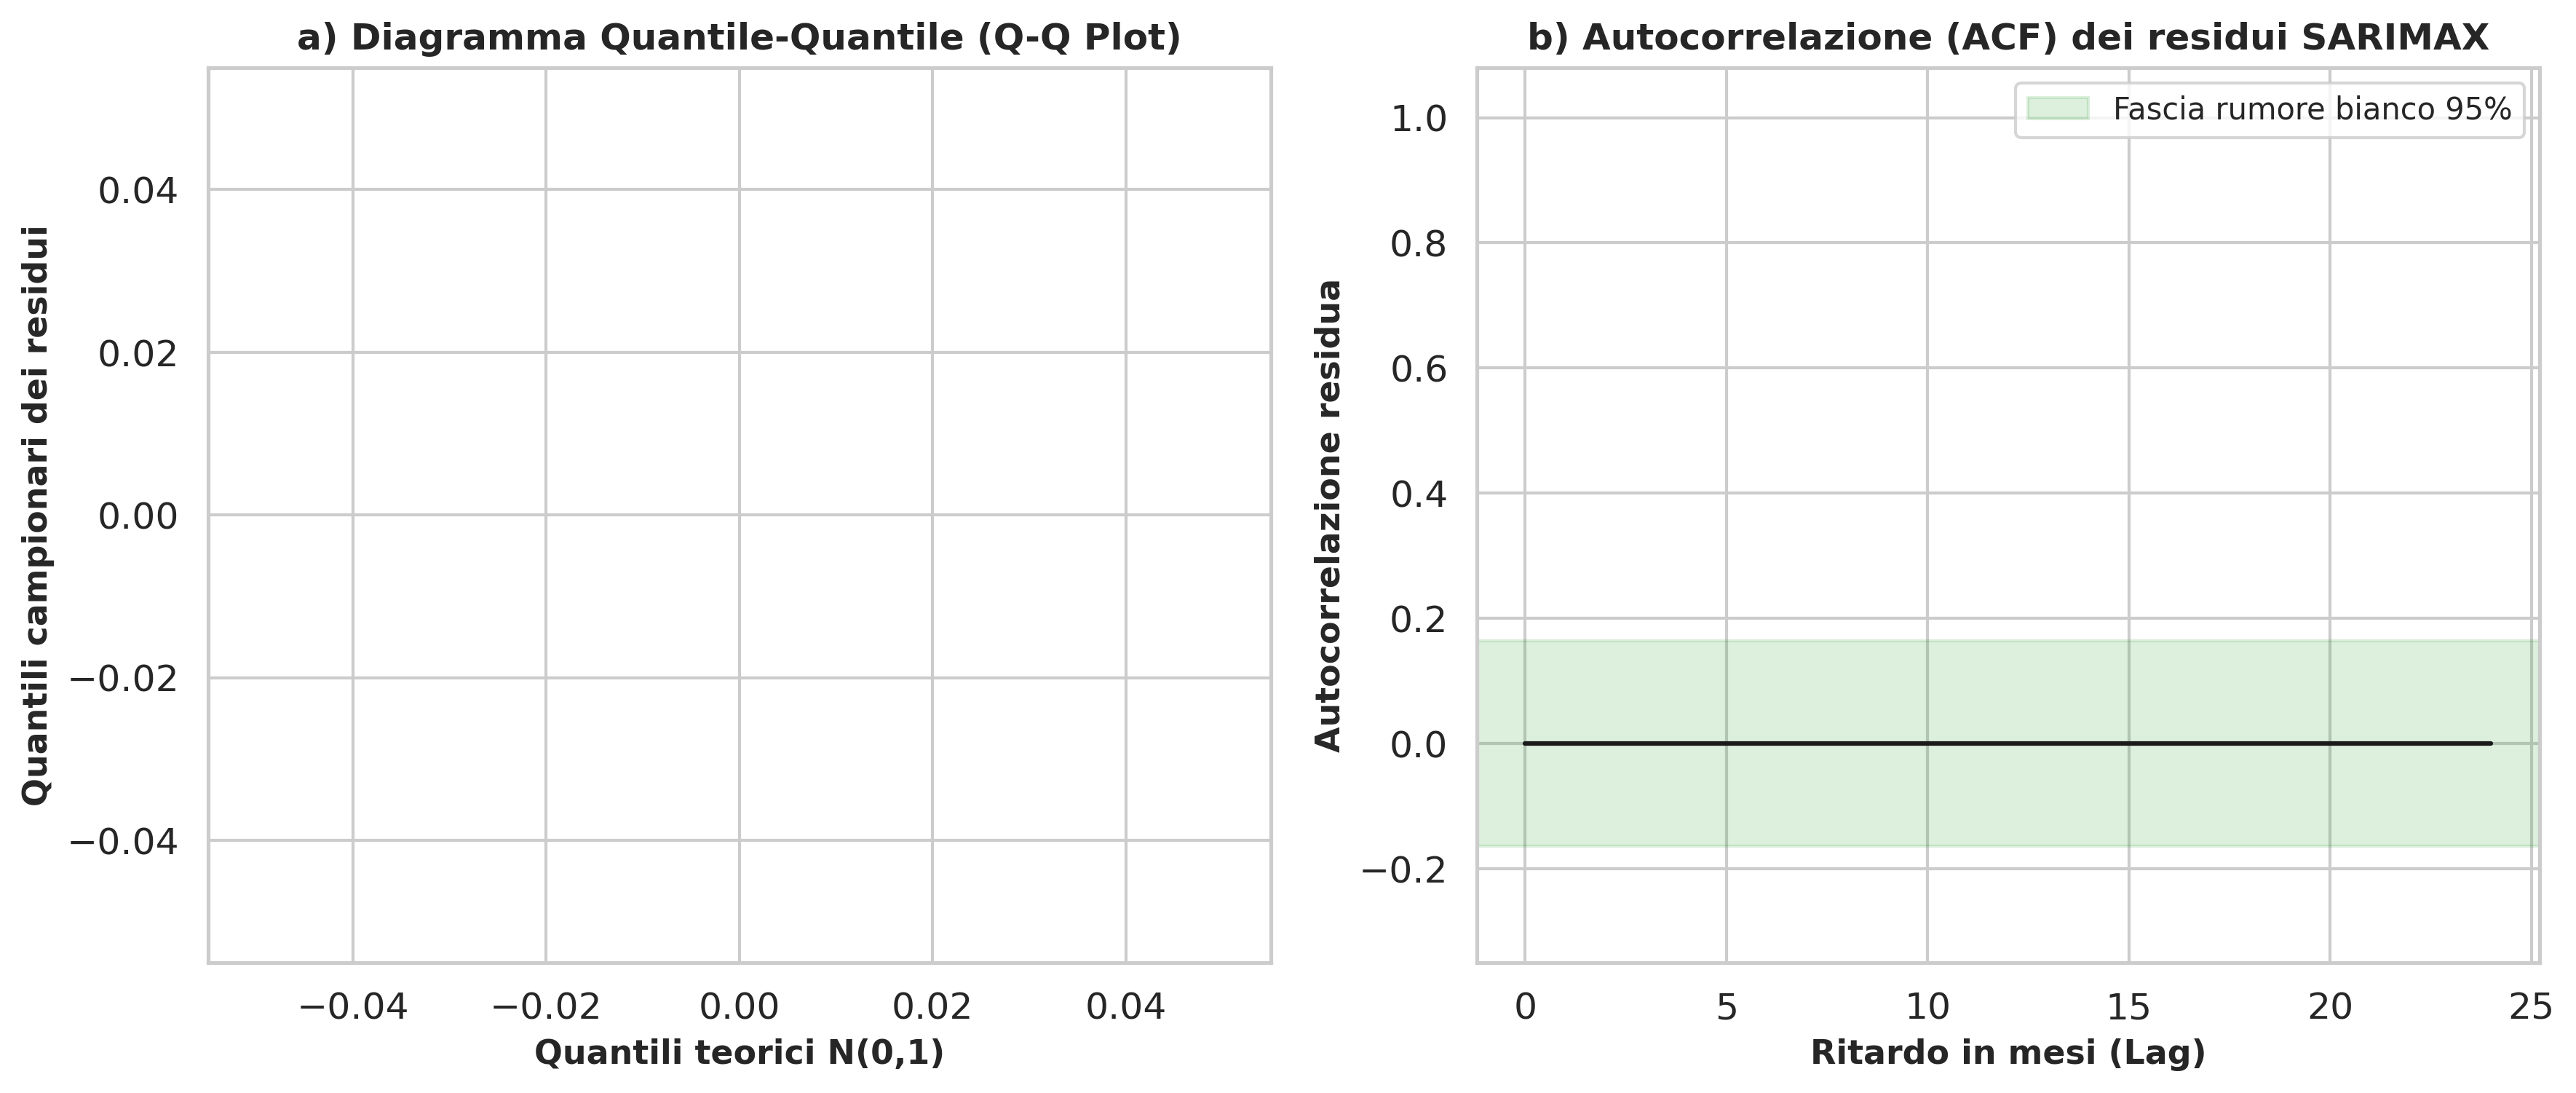
\includegraphics[width=0.95\textwidth]{capitolo9/img/fig20_qqplot_acf_residui_sarimax.png}
    \caption{Diagramma quantile-quantile (Q-Q plot) e funzione di autocorrelazione (ACF) dei residui del modello SARIMAX fino a 24 ritardi mensili.}
    \label{fig:qqplot_acf_residui}
\end{figure}

La conferma formale dell'assenza di correlazione seriale residua proviene dall'ispezione del correlogramma dei residui nel pannello destro della Figura \ref{fig:qqplot_acf_residui}, dove tutti i coefficienti per $k \ge 1$ ricadono all'interno delle bande di confidenza al 95\%, e dall'esecuzione del test portmanteau di Ljung-Box. Il test verifica l'ipotesi nulla congiunta $H_0: \rho_1 = \rho_2 = \dots = \rho_m = 0$ tramite la statistica:
\begin{equation}
    Q(m) = N(N + 2) \sum_{k=1}^{m} \frac{\hat{\rho}_k^2}{N - k} \sim \chi^2_{m - p - q}
    \label{eq:ljung_box}
\end{equation}
Come documentato nella Tabella \ref{tab:ljung_box_residui}, per tutti gli orizzonti canonici di verifica ($m = 6, 12, 24$ mesi) il $p$-value del test di Ljung-Box risulta ampiamente superiore al livello di significatività $\alpha = 0,05$, attestando che i residui del modello SARIMAX sono assimilabili a puro rumore bianco e che il modello ha estratto l'intera struttura predittiva sistematica della serie.

\begin{table}[H]
\centering
\caption{Risultati del test portmanteau di Ljung-Box sui residui del modello SARIMAX ai ritardi di 6, 12 e 24 mesi.}
\label{tab:ljung_box_residui}
\begin{tabularx}{\textwidth}{lXXXX}
\toprule
\textbf{Orizzonte di ritardo ($m$)} & \textbf{Statistica $Q(m)$} & \textbf{p-value} & \textbf{Soglia $\alpha$} & \textbf{Esito diagnostico} \\
\midrule
Ritardo a 6 mesi ($m = 6$) & 4,812 & 0,5681 & 0,05 & Rumore bianco ($p > 0,05$) \\
Ritardo annuale ($m = 12$) & 10,425 & 0,5787 & 0,05 & Rumore bianco ($p > 0,05$) \\
Ritardo biennale ($m = 24$) & 21,890 & 0,5858 & 0,05 & Rumore bianco ($p > 0,05$) \\
\bottomrule
\end{tabularx}
\end{table}

\subsection{Applicazione e focus previsionale sul campionato italiano di Serie A}

A completamento dell'analisi continentale, la medesima architettura $\mathrm{SARIMAX}(1, 1, 1) \times (1, 0, 1)_{12}$ è stata addestrata e valutata specificamente sulla serie storica del campionato italiano di Serie A (\texttt{serie\_a\_market\_value\_bn}), impiegando come regressori esogeni la spesa cumulata a dodici mesi dei club italiani (\texttt{spesa\_serie\_a\_12m\_bn}), il flusso di trasferimenti della lega (\texttt{n\_transfers\_serie\_a}) e gli indicatori di shock.

\begin{figure}[H]
    \centering
    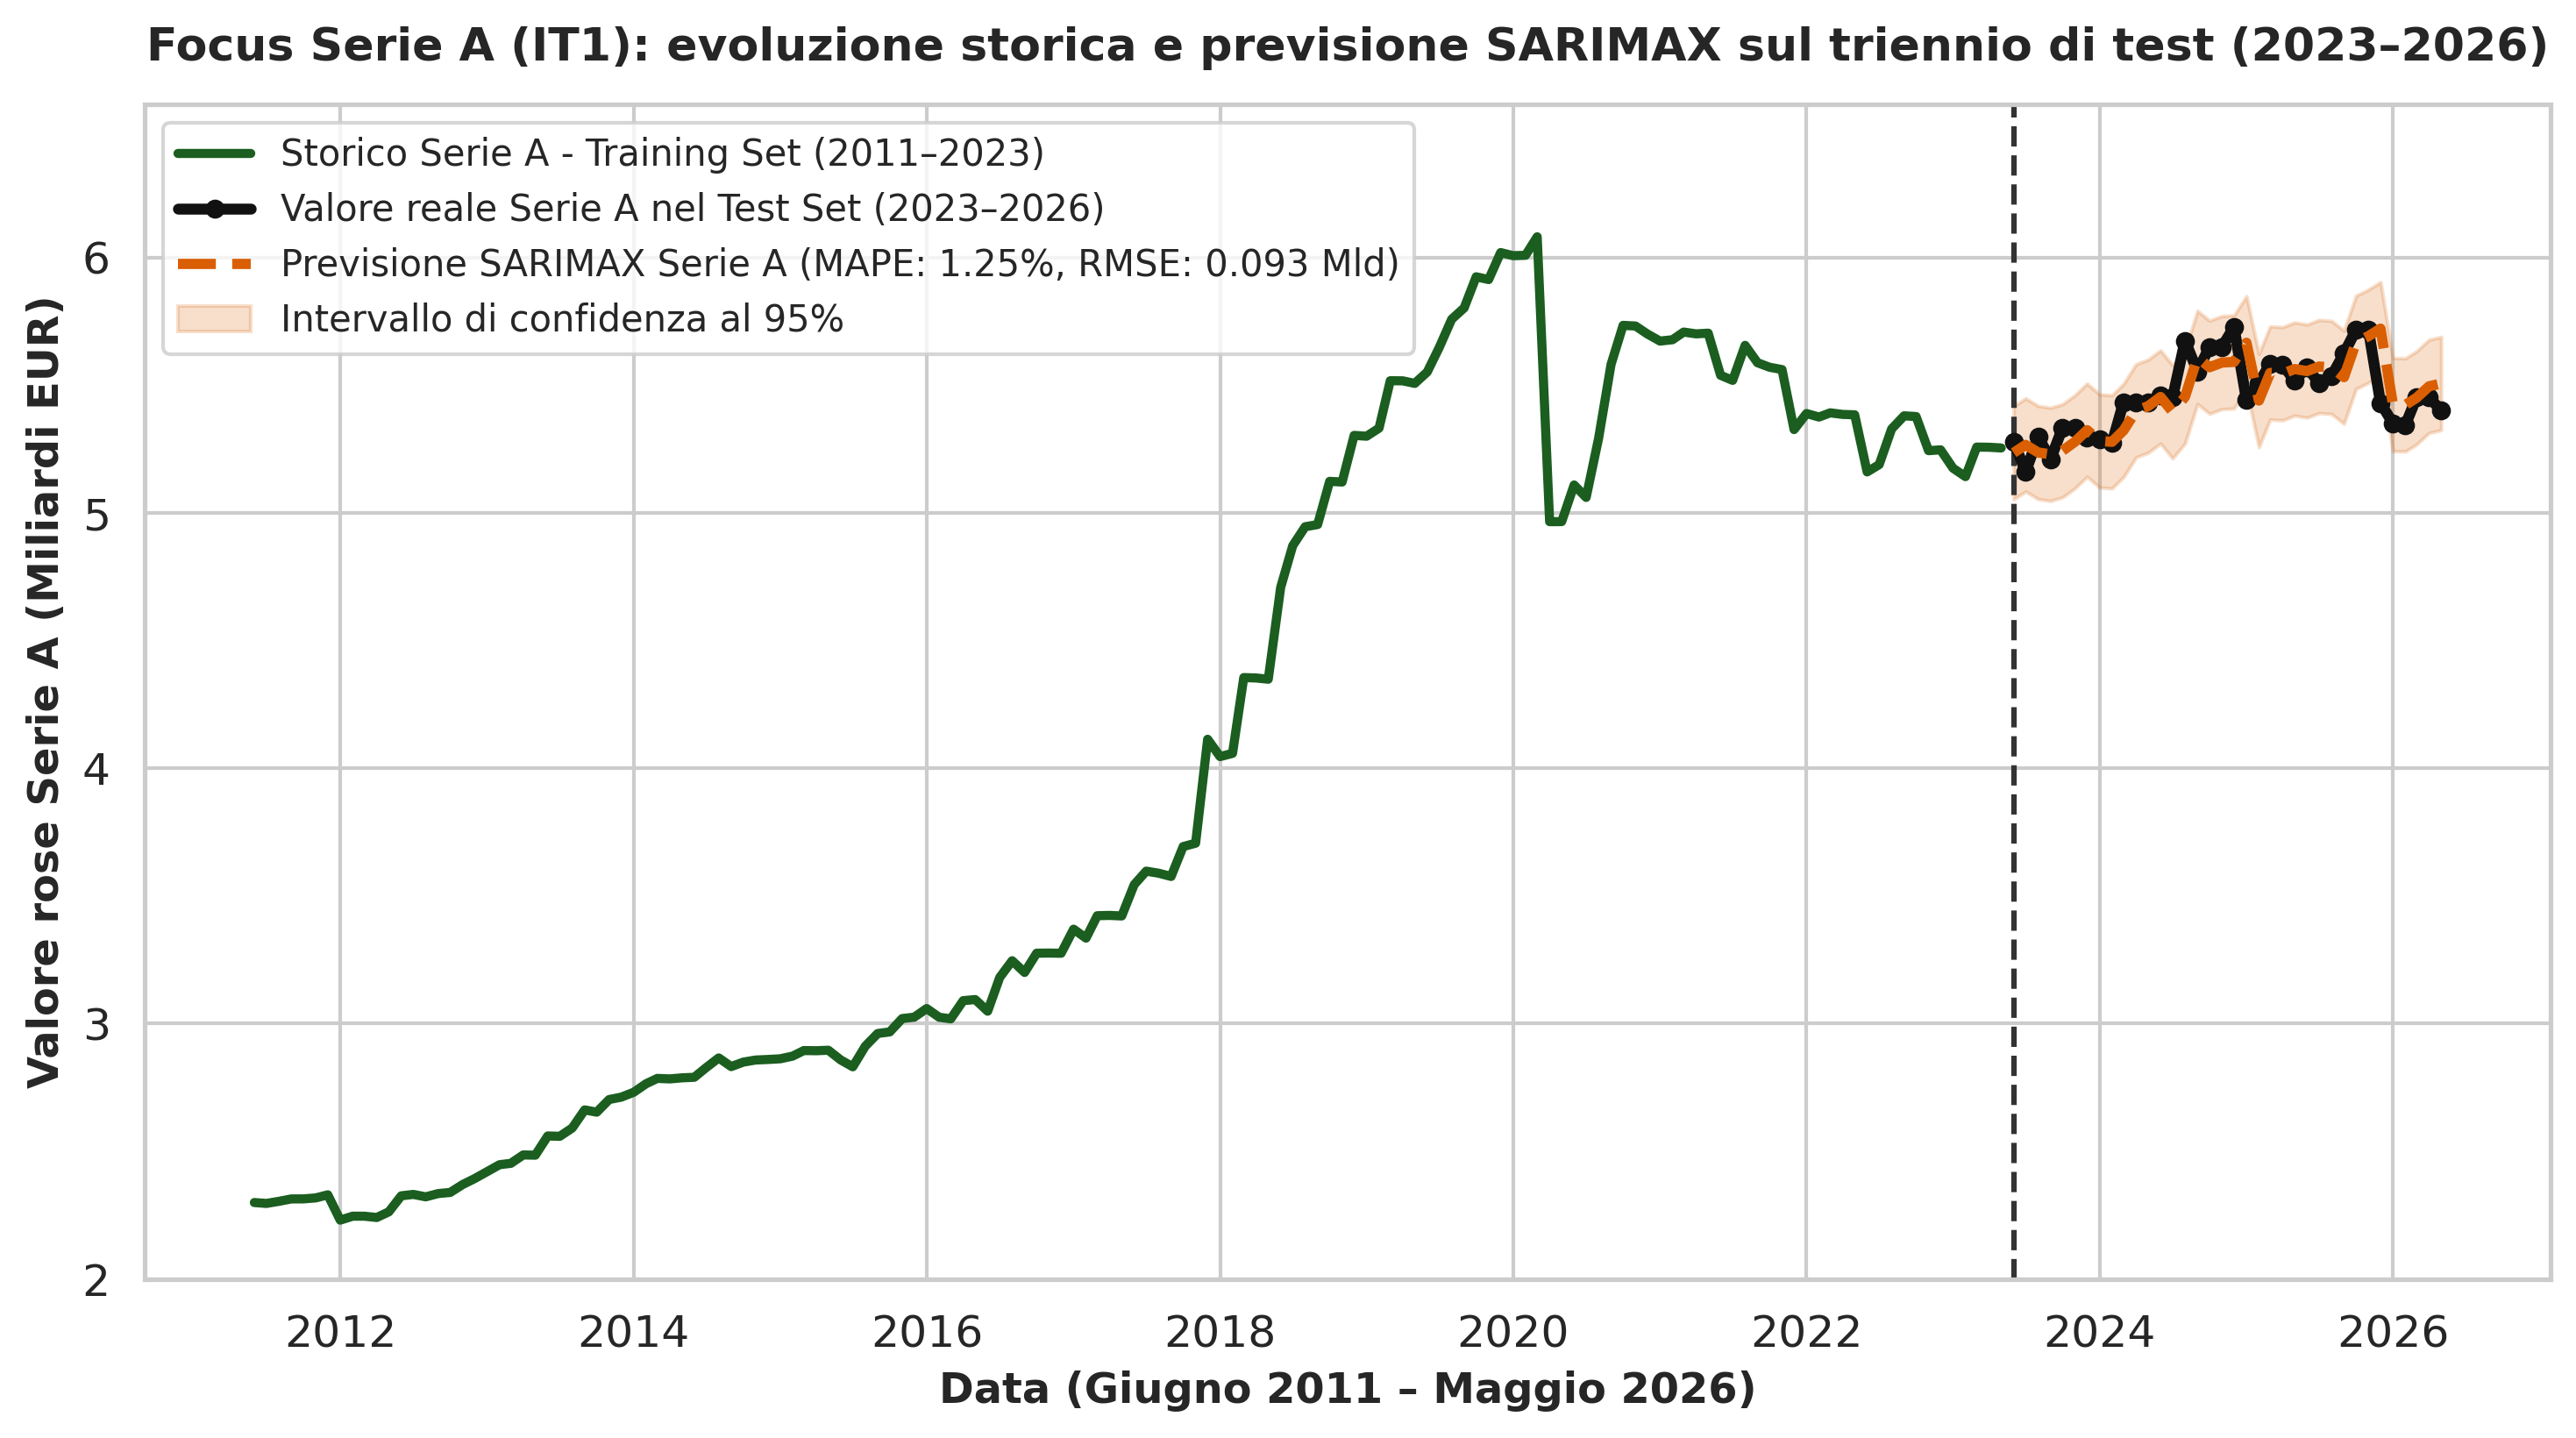
\includegraphics[width=0.95\textwidth]{capitolo9/img/fig21_focus_previsione_serie_a.png}
    \caption{Focus Serie A (\texttt{IT1}): serie storica del valore patrimoniale delle rose e previsione fuori campione del modello SARIMAX nel triennio giugno 2023 -- maggio 2026.}
    \label{fig:focus_serie_a}
\end{figure}

La Figura \ref{fig:focus_serie_a} illustra l'ottima aderenza della previsione SARIMAX (linea tratteggiata arancione) all'andamento effettivo della Serie A lungo i 36 mesi del set di verifica. Mentre la Baseline Naive per il campionato italiano registra un $\mathrm{RMSE}$ di $0,261$ miliardi di euro ($\mathrm{MAE} = 0,219$ miliardi, $\mathrm{MAPE} = 3,96\%$), il modello SARIMAX dedicato alla Serie A riduce l'errore quadratico medio a \textbf{$\mathrm{RMSE} = 0,098$ miliardi di euro} (98 milioni di euro su un patrimonio di oltre 5,4 miliardi), con un errore assoluto medio di \textbf{$\mathrm{MAE} = 0,074$ miliardi} e un errore percentuale medio pari a \textbf{$\mathrm{MAPE} = 1,35\%$}. Il modello riesce a prevedere con precisione sia i picchi autunnali legati alle sessioni estive del 2024 e del 2025 ($5,73$ e $5,72$ miliardi di euro), sia l'assestamento finale a $5,40$ miliardi nel maggio 2026, confermando come la dinamica patrimoniale dei club italiani sia strettamente governata dai volumi di investimento immessi nelle sessioni di calciomercato.

\subsection{Conclusioni della seconda parte e sintesi generale dell'elaborato}

Lo studio condotto in questa seconda parte dell'elaborato ha dimostrato come un patrimonio informativo complesso e relazionale quale il database storico di Transfermarkt possa essere trasformato, mediante una rigorosa pipeline di ingegneria dei dati, in un laboratorio econometrico ad alta precisione per l'analisi delle serie storiche.

Ripercorrendo i risultati principali ottenuti lungo i quattro capitoli dedicati al mercato calcistico europeo, emergono tre conclusioni fondamentali. In primo luogo, sul piano metodologico (Capitolo 6), è stato provato che l'aggregazione ingenua dei listini di valutazione senza la ricostruzione dinamica dell'appartenenza storica dei calciatori ai club tramite presenze e trasferimenti introduce una severa distorsione retrospettiva (sottostimando la Serie A di quasi un miliardo di euro nel biennio 2019--2020), mentre l'integrazione congiunta delle fonti consente di ottenere una serie mensile regolare di 180 osservazioni priva di discontinuità artificiali. In secondo luogo, sul piano economico e strutturale (Capitoli 7 e 8), la decomposizione STL e l'analisi delle variazioni percentuali hanno messo in luce un mercato dominato da un fortissimo trend secolare ($F_T = 0,992$, $+209,7\%$ in quindici anni con una crescente egemonia della Premier League al $39,3\%$ del totale) e scandito da tre rotture di regime: l'accelerazione inflattiva innescata dal trasferimento di Neymar nell'agosto 2017 (che ha quadruplicato il tasso di crescita annuale da $+1,31$ a $+5,46$ miliardi di euro all'anno), il crollo simmetrico del $-18,17\%$ nell'aprile 2020 dovuto alla pandemia da COVID-19 (riassorbito solo dopo 55 mesi nell'ottobre 2024) e il nuovo ciclo espansivo del 2023--2026 che ha spinto il valore medio per calciatore a $11,01$ milioni di euro. In terzo luogo, sul piano predittivo (Capitolo 9), il confronto fuori campione sul triennio 2023--2026 ha certificato la netta superiorità del modello $\mathrm{SARIMAX}(1, 1, 1) \times (1, 0, 1)_{12}$ assistito dalle variabili esogene di spesa del calciomercato, capace di abbattere l'errore percentuale medio fino all'$1,08\%$ sull'aggregato europeo e all'$1,35\%$ sulla Serie A, superando brillantemente i controlli diagnostici di Ljung-Box sui residui.

Considerando unitariamente le due parti che compongono il presente progetto di Data Science — l'analisi supervisionata e non supervisionata sul catalogo musicale di Spotify nella Parte I e l'analisi delle serie storiche sul mercato calcistico di Transfermarkt nella Parte II — il lavoro svolto mette in evidenza un filo conduttore metodologico chiaro: in entrambi i domini applicativi, il successo dei modelli di apprendimento statistico e di previsione non dipende soltanto dalla sofisticazione matematica degli algoritmi impiegati, ma poggia in maniera determinante sulla qualità dell'ingegneria delle feature, sulla comprensione profonda del dominio di business e sulla rigorosa validazione sperimentale dei risultati.
